\chapter{Compile-Time PLT Redex Representation}
\label{chapter05}

This chapter describes how PyPltRedex represents the constructs of PLTRedex that were described in Section \ref{01-pltredex} and establishes the notation that will be used throughout the report. Forms that are not part of PLTRedex are also introduced.

\section{Pattern Language}

This section describes the subset of PLTRedex's pattern specification language supported by \texttt{PyPltRedex}. Grammar for the pattern language can be seen in Figure \ref{pattern-grammar}, in EBNF notation. 

\begin{figure}[h]
\begin{minted}[tabsize=2,obeytabs,escapeinside=//,mathescape=true,fontsize=\normalsize]{text}
pattern = number 
        | integer 
        | real 
        | natural 
        | string 
        | boolean 
        | variable-not-otherwise-mentioned 
        | hole 
        | symbol
        | (in-hole pattern pattern)
        | (pattern-sequence *) 

pattern-sequence : pattern 
                 | pattern ...  # literal ellipsis
\end{minted}
\caption{Grammar of the pattern language.}
\label{pattern-grammar}
\end{figure}

\begin{itemize}
\item
\textit{number} pattern matches any number.

\item
\textit{integer} matches any exact integer. 

\item
\textit{real} matches any real number.

\item
\textit{natural} matches any natural number; that is, any non-negative integer.

\item
\textit{string} matches any string.

\item
\textit{boolean} matches any boolean \texttt{\#t} or \texttt{\#f}.
\item
\textit{variable-not-otherwise-mentioned} matches any symbol that is not used as a literal in the language definition. For example, if language definition contains the pattern \texttt{(+ number number)} \textit{variable-not-otherwise-mentioned} will not match symbol \texttt{+}.

\item
\textit{hole} matches \texttt{hole} term exactly.

\item
\textit{symbol} matches any symbol except if its value coincides with non-terminal symbol in the language definition or contains an underscore.
\end{itemize}

All patterns above, except \textit{hole} can be suffixed with underscore and identifier (for example, \textit{number\_1}) to create a binding to a matched term.

\begin{itemize}
\item
\textit{(in-hole pattern pattern)} traverses the term trying to match the second pattern; upon successful match the term matching the second pattern is replaced with the term \texttt{hole} and then the first pattern is matched. The first pattern must match exactly one hole.

\item
\textit{pattern-sequence} pattern matches a term list, where each pattern-sequence element matches an element of the list. Each individual pattern within the sequence can be suffixed with \texttt{...} (literal ellipsis) and that will match zero or more terms matching the pattern.

Ellipses may produce non-deterministic matches. For example, consider a pattern \texttt{(number\_1\ ...\ number\_2\ ...)} and a term \texttt{(1 2)}. There are three resulting matches: 
\begin{itemize}
	\item \texttt{(number\_1:\ (), number\_2:\ (1 2))}
	\item \texttt{(number\_1:\ (1), number\_2:\ (2))}
	\item \texttt{(number\_1:\ (1 2), number\_2:\ ())}
\end{itemize}
		
In the first case, \texttt{number\_1 ...} matches zero terms that match the pattern \texttt{number\_1} and hence pattern \texttt{number\_2\ ...} has to match remaining numbers. In the second case, \texttt{number\_1\ ...} matches a term \texttt{1}, and hence the term \texttt{2} is matched by \texttt{number\_2 ...}. Lastly, \texttt{number\_1\ ...} may match all the numbers in the sequence, leaving nothing for \texttt{number\_2\ ...} to consume.
\end{itemize}

If patterns in the pattern-sequence are suffixed with the same identifier (e.g. \texttt{(number\_1 number\_1)})), then the match is constrained to terms that are equal. That means term \texttt{(1 1)} matches the pattern but \texttt{(1 2)} does not. For patterns in a \texttt{define-language} form constraint checking is not performed. PLTRedex provides other constraint checks but they will not be considered.

\section{Compile-Time Representation of Patterns}

Throughout the report the following notation will be used to represent the Python classes used in the implementation of the pattern language. It follows the following format: \mintinline{text}{Typename(|$a$|: A, [|$b_1,...,b_n$|]: B, [|$c_1,...,c_m$|]: C?)}. $a$ is a field of type \texttt{A}. \mintinline{text}{[|$b_1,...,b_n$|]} is a sequence containing $n$ fields of type \texttt{B}. \mintinline{text}{[|$c_1,...,c_m$|]} is a sequence containing \textit{zero} or $m$ fields of type \texttt{C} (that is, \texttt{C?} is an optional type).

\begin{figure}[ht]
	\centering
	\makebox[\textwidth][c] { 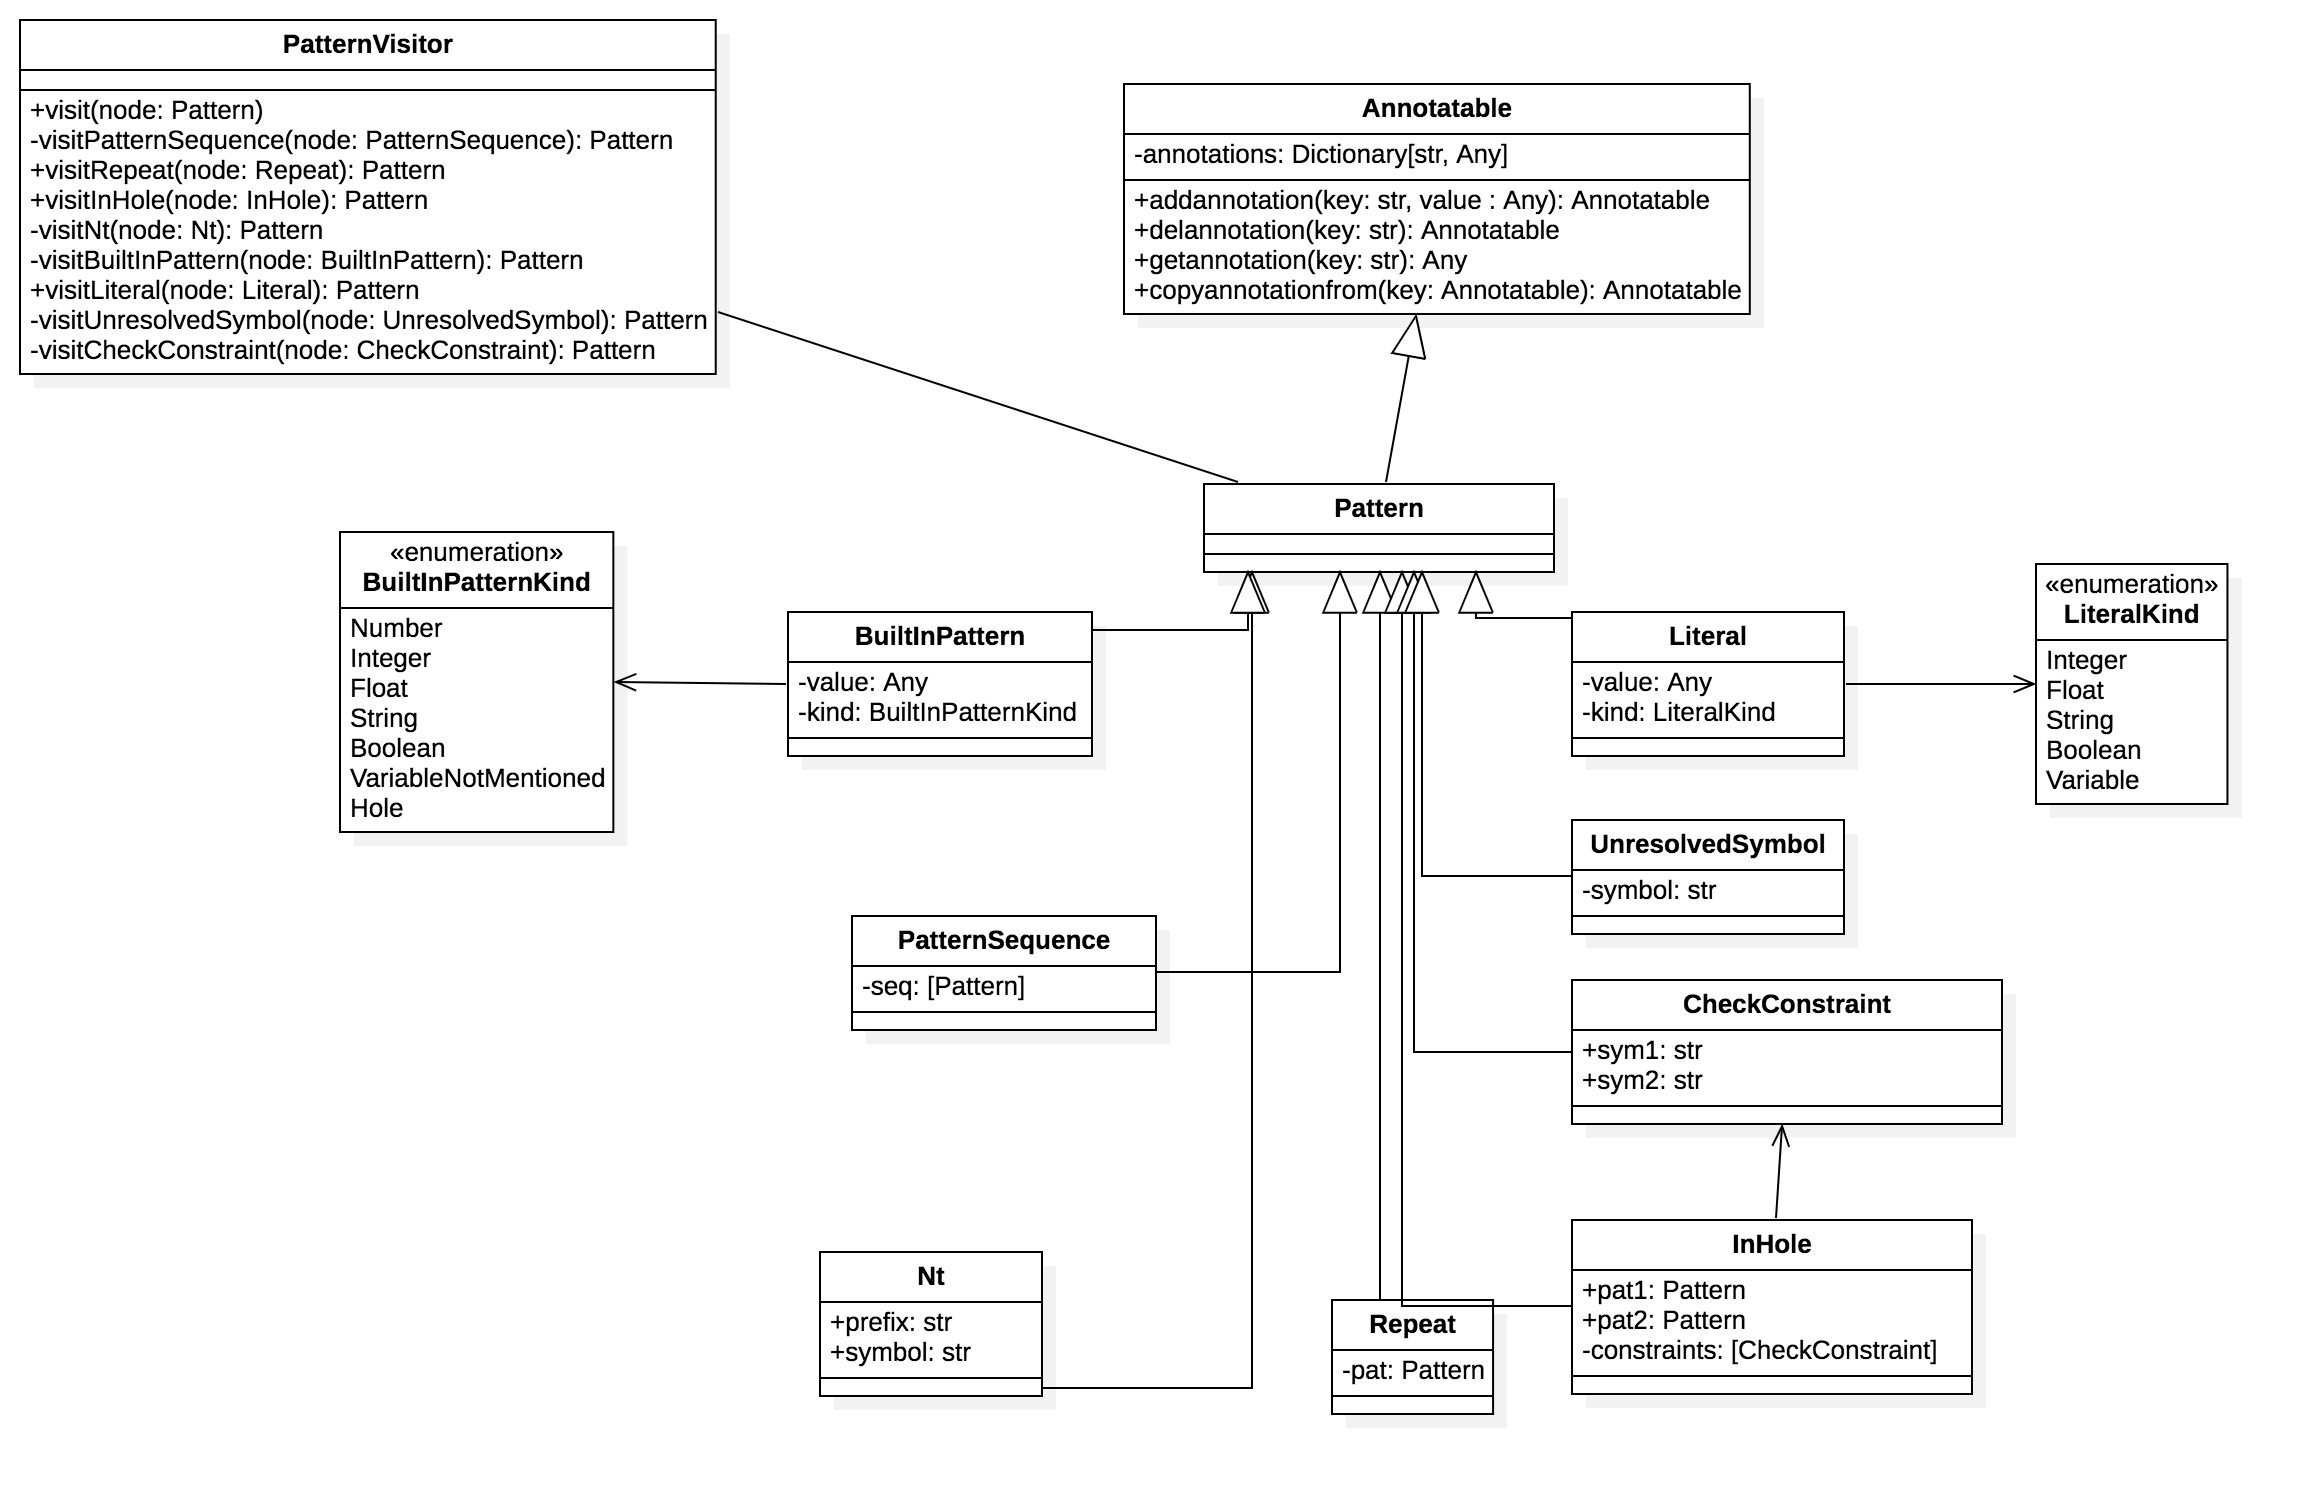
\includegraphics[scale=0.23]{class-diagram-pattern.png} }
	\caption{Representation of patterns.}
\label{class-diagram-pattern}
\end{figure}

Figure \ref{class-diagram-pattern} shows class diagram for all patterns.

\begin{itemize}
\item
\PatternSequence \space represents the \texttt{pattern-sequence} clause of the pattern language and may contain zero or more child patterns $p_i$. 

\item 
\PatternRepeat \space represents pattern $p_r$ under ellipsis.

\item
\PatternCheckConstraint is used for equality checking of terms. Terms assigned to $sym_1$ and $sym_2$ are checked for equality.

\item 
\NonTerminal \space represents non-terminal. $nt$ is a non-terminal symbol, while $pv$ is a pattern-variable to which some term will be assigned during matching. 

\item
\BuiltInPattern \space represents various built-in patterns such as \texttt{number} or \texttt{string}. $tag$ is chosen from \texttt{BuiltInPatternKind} enumeration.

\item
\PatternInHole \space represents \texttt{in-hole} pattern where $p_1$ and $p_2$ are patterns, and $c_1, ..., c_n$ are optional \ConstraintCheckNoArg \space instances.

\item 
\LiteralPattern \space represents a literal value seen in a pattern. Its $kind$ is chosen from \texttt{PatternLiteralKind} enumeration and $v$ is the value of the literal. The type of the literal must match the $kind$.

\item 
\UnresolvedSymbol is used to represent symbols that are initially unknown to be non-terminal, built-in pattern, or literal; $sym$ is the symbol.

\end{itemize}

\section{Term-Templates}
\label{section:term-templates}

The compile-time representation of terms differs greatly from the runtime representation described previously. The reason for this is the necessity to handle ellipses; or, more specifically, the substitution of pattern variables under ellipses - \texttt{PLTRedex} handles this dynamically and erroneous ellipses aren't detected until term creation time.
It is desirable to handle ellipsis depth checking of pattern variables at compile time to be able to provide compile time error messages. Doing this allows for the complete elimination of ellipses from the runtime (with variable \texttt{...} being a reserved symbol that throws an Exception). In addition, this also allows for the detection of metafunction applications statically.

The grammar for terms can be seen in Figure \ref{termtemplate-grammar}. To differentiate between runtime terms, the compile-time representation of terms will be called \textbf{term-templates}.

\begin{figure}
\begin{minted}[tabsize=2,obeytabs,escapeinside=//,mathescape=true,fontsize=\normalsize]{text}
term-template = pattern-variable
              | (term-sequence *)
              |,(functionname term*)
              |(in-hole term term)
              | hole
              | integer
              | float
              | string
              | boolean
term-sequence = term
              | term ... ; literal ellipsis
              | ,@(function term *)
\end{minted}
\caption{Grammar for term-templates.}
\label{termtemplate-grammar}
\end{figure}

\begin{itemize}
\item
\texttt{pattern-variable} represents pattern variables.
\item
\texttt{,(functionname term*)} calls a user-implemented RPython function with zero or more terms as arguments.
\item
\texttt{,@(functionname term*)} calls a user-implemented RPython function with zero or more terms as arguments that must return a list. The content of the returned list are then inserted into term-sequence at that position.
\item
\texttt{(in-hole term term)} locates \lstinline{hole} in the first term and replaces it with the second term.
\item
\texttt{hole} represents the term \lstinline{hole}
\item
\texttt{integer} represents any literal integer.
\item
\texttt{float} represents any literal floating point number.
\item
\texttt{string}  represents any literal string.
\item
\texttt{boolean}  represents any literal boolean.
\item
	\texttt{term-sequence} represents a list of term-templates.  Each individual term-template within the sequence can be suffixed with \texttt{...} (literal ellipsis) indicating the ellipsis depth of some pattern-variable in that term-template.
\end{itemize}

\section{Compile-time Representation of Term-Templates}

Throughout the report the following notation will be used to represent actual Python classes used to implement the term-templates.

\begin{figure}[ht]
	\centering
	\makebox[\textwidth][c] { 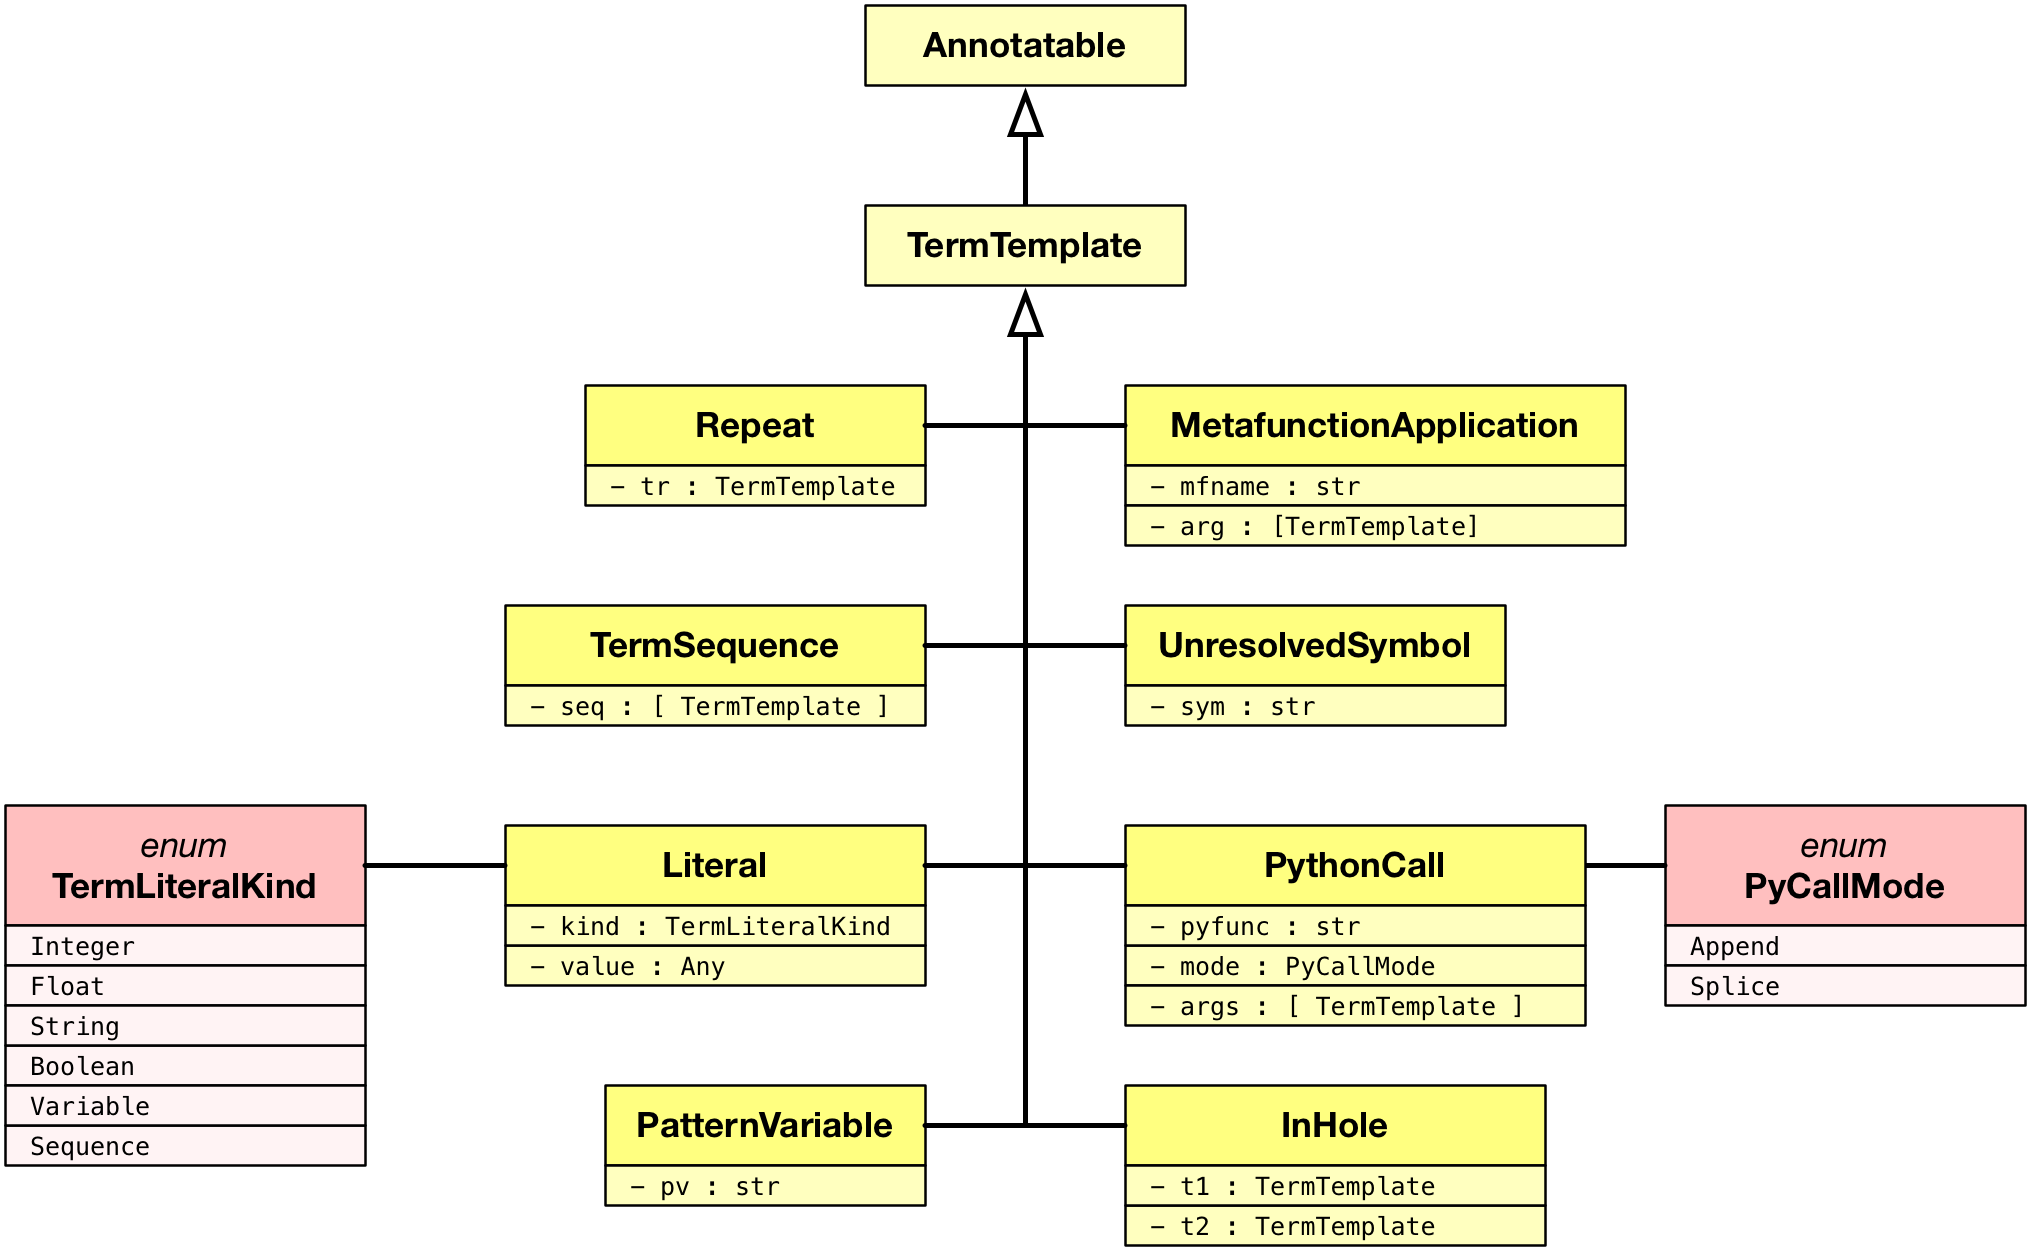
\includegraphics[scale=0.19]{class-diagram-termtemplate.png} }
	\caption{Representation of term-templates.}
\label{class-diagram-termtemplate}
\end{figure}

Figure \ref{class-diagram-termtemplate} shows class diagram for all term-templates.


\begin{itemize}
\item \TermSequence \space represents term-template sequences and may contain zero or more child term-templates $t_i$.
\item \TermRepeat \space represents a term-template under ellipsis.
\item \TermInHole \space represents \texttt{in-hole} term-template
\item \PythonCall \\ represents \texttt{,(functionname term*)} and \texttt{,@(functionname term*)} term-template. $mode$ is used to indicate which one of those it is - $m$ is set to \texttt{Normal} if it is the first, otherwise \texttt{Splice} if it is the latter. $pyfunc$ is expected to be a defined RPython-compatible function.
\item \TermLiteral \space represents any literal. It is initialized with the appropriate tag.
\item \PatternVariable \space represents all pattern-variables.
\item \UnresolvedSymbol \space represents unresolved symbols. Initially it is unknown if a symbol is a pattern-variable or a literal.
\end{itemize}

\section{Top-Level Forms}

\mbox{PyPltRedex supports three primary forms. \texttt{define-language} and \texttt{define-metafunction}} forms are lifted directly PLTRedex. \texttt{reduction-relation} form had to be modified resulting in \texttt{define-reduction-relation}. \texttt{read-from-stdin-and-apply-reduction-relation*} form  is based on  \texttt{apply-reduction-relation} but instead it reads a term from standard input, parses it, and only then applies reduction relation. The grammar for these forms can be found in Figure \ref{grammar-tlmain}.

\begin{figure}
\begin{minted}[tabsize=2,obeytabs,escapeinside=//,mathescape=true,fontsize=\normalsize]{text}
define-language = ( define-language language-name non-terminal-definition+ )
non-terminal-definition = ( non-terminal-name ::= pattern+ )

define-metafunction = ( define-metafunction language-name metafunction-contract metafunction-case+ )
metafunction-contract =	id : pattern-sequence* -> pattern
metafunction-case =  [( name pattern* ) term-template]

reduction-relation = ( define-reduction-relation name language domain reduction-case+ )
reduction-case = (-> pattern term-template reduction-case-name)
domain = #:domain pattern

read-from-stdin-and-apply-reduction-relation = ( read-from-stdin-and-apply-reduction-relation :#mf metafunction-name )
\end{minted}
\caption{Grammar for primary top-level forms.}
\label{grammar-tlmain}
\end{figure}

\begin{itemize}
\item
\TlDefineLanguage. $n$ is the name of the language and $nt_1,...,nt_m$ are \NtDefinitionN \space instances containing one or more \texttt{Pattern} instances.

\item
\TlDefineMetafunction. $n$ is the \texttt{id} specified by \texttt{metafunction-contract}. Let $p_1, ..., p_n$ be the pattern sequence specified by the \texttt{metafunction-contract}, between \texttt{id} and \texttt{->}. $domain$ pattern is then constructed in the following way: \mintinline{text}{PatternSequence(|$n$|, [|$p_1$|, |$...$|, |$p_n$|])}. $codomain$ pattern is the one following \texttt{->}. If input term doesn't match pattern $domain$, an Exception is raised. Similarly, if the resulting term doesn't match $codomain$ pattern, an Exception is also raised. If metafunction produces no terms, an Exception is raised. $mc_1,...,mc_n$ is the sequence of \space \MetafunctionCase \space containing the pattern $p$ to be matched and the term-template $t$ to plug matches into. $l$ is the name of the language with respect to which all non-terminal symbols in patterns $p$ are resolved.

\item \TlDefineReductionRelation. $n$ is the name of the reduction-relation; an optional $domain$ pattern ensures that the input term and resulting terms match the pattern otherwise an Exception is raised, and each $rc_i$=\ReductionCase \space contains a pattern $p$ and term-template $t$; $n$ is the name of the reduction case.

This form had to be modified due to the fact that PyPltRedex doesn't interpret Racket in any way and thus \texttt{define} form is not supported. Therefore, \texttt{define} and \texttt{reduction-relation} forms had to be collapsed into a single \texttt{define-reduction-relation} form.

\item \ReadFromStdinAndApplyReductionRelation \space is self-explanatory -  it reads a string from a standard input or file, parses it into a term using logic outlined in Section \ref{section:lex-parse}, and applies a reduction-relation with name $r$. Optionally, one can provide the metafunction with a name $f$ to apply to the parsed term before application of $r$. This allows for separation of the specification of "code" from everything else that is required to evaluate the "code" (such as model of the heap/stack, etc).
\end{itemize}

PyPltRedex provides several additional forms with testing functionality. The goal is to run individual components of PyPltRedex, such as the pattern matcher and term generator, and then compare the results against expected ones. These additional forms are \texttt{redex-match-assert-equal}, \texttt{term-let-assert-equal} and \\ \texttt{apply-reduction-relation-assert-equal}.

\begin{itemize}
\item \RedexMatchAssertEqual. Given a term instantiated from term-template $t$, it is matched against a pattern $p$ containing non-terminal symbols from language $l$. A resulting list of matches is then compared against the list of expected matches $m_1,...,m_n$, potentially empty, where $m_i=$\space\Match. The term instantiated from term-template $t_i$ is assigned to pattern-variable $s_i$. An Exception is raised under the following conditions:
	\begin{enumerate}
	\item Lengths of both lists do not match.
	\item Given two matches from both lists at position $i$, $m_i^{expected} \neq m_i^{actual}$, with the equality operation defined in Section \ref{section:Match}.
	\end{enumerate}
	This form is based on the \texttt{redex-match} form provided by PLTRedex.

\item \TermLetAssertEqual. Given a list of pattern-variable assignments $(v_i, n_i, t_i)$, a new \texttt{Match} instance is created, the term instantiated from the term-template $t_i$ is assigned to the pattern-variable $v_i$. The resulting \texttt{Match} is then plugged into term-template $t$, and the resulting term is compared against a term produced by term-template $e$.

\item \ApplyReductionRelationAssertEqual. This form takes a term produced by the term-template $t$, applies reduction relation with name $r$, and then compares resulting terms against a list of terms instantiated from term-templates $e_1,...,e_n$.
	\begin{enumerate}
	\item Lengths of both lists do not match.
	\item Given two terms from both lists at position $i$, $t_i^{expected} \neq t_i^{actual}$, with equality operation defined in Section \ref{section:runtime-terms}
	\end{enumerate}
\end{itemize}

Figure \ref{class-diagram-toplevel} shows class diagram for all top-level forms.

\begin{figure}[htb]
	\centering
	\makebox[\textwidth][c] { 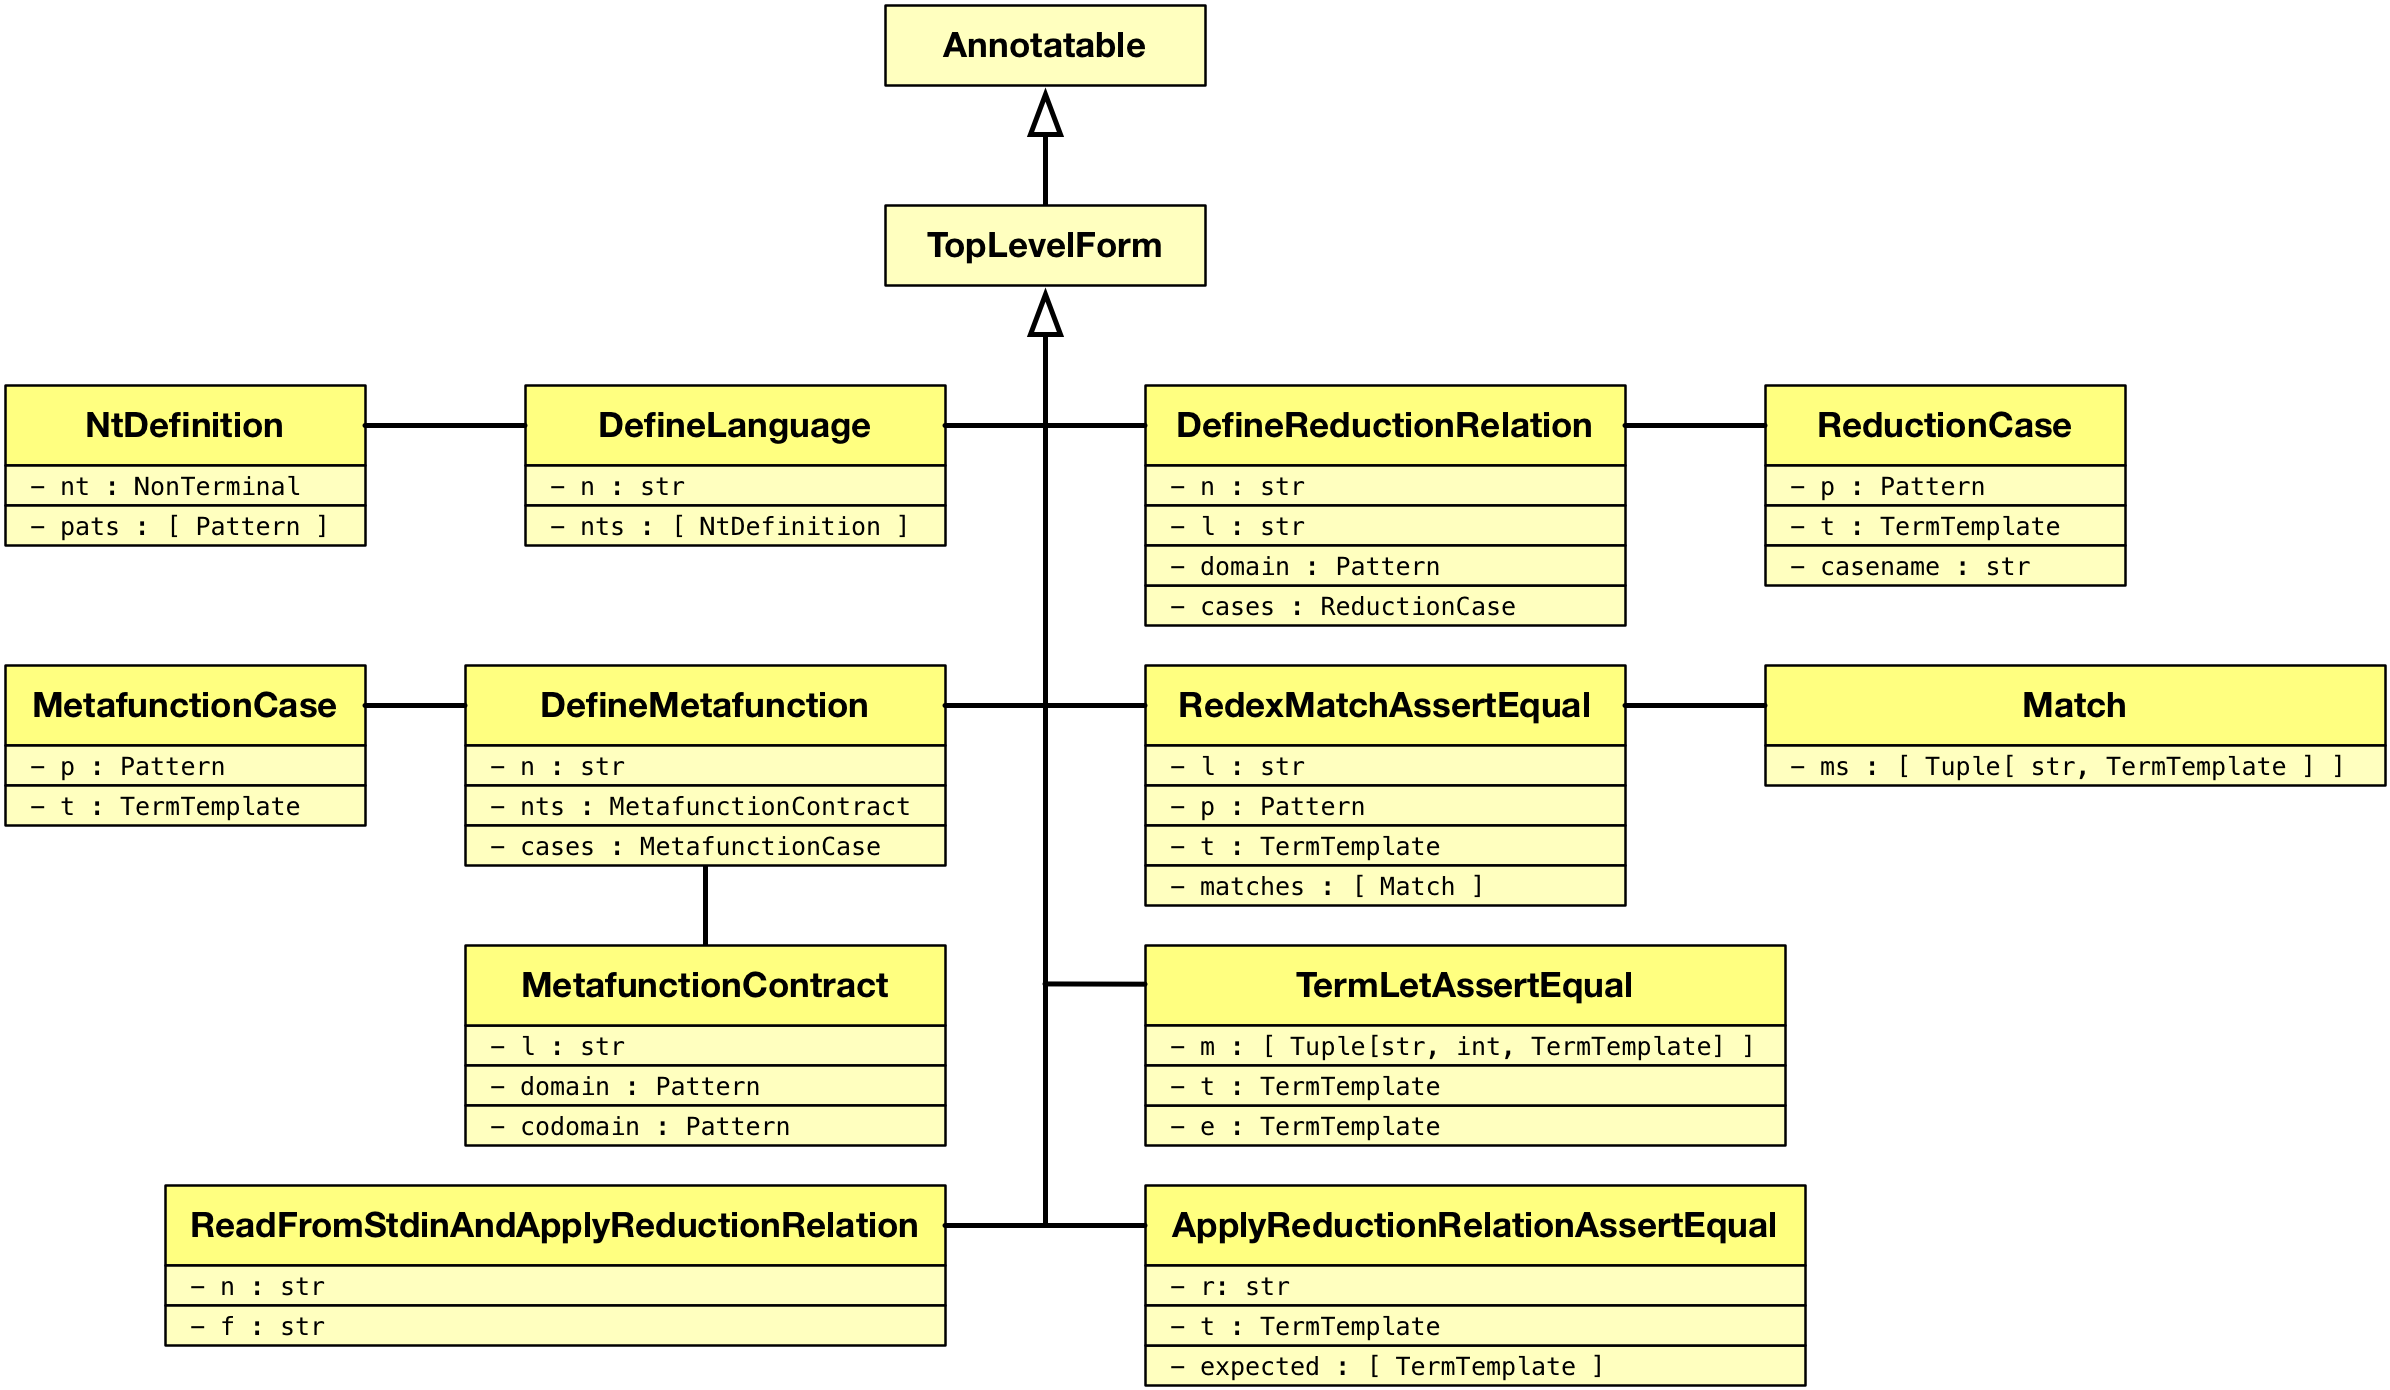
\includegraphics[scale=0.21]{class-diagram-toplevel.png} }
	\caption{Representation of top-level forms.}
\label{class-diagram-toplevel}
\end{figure}

\section{Visitors}
\label{section:visitors}
Since patterns, term-templates, and top-level forms require analysis or transformations applied to them, visitors for each \texttt{TermTemplate}, \texttt{Pattern} and \texttt{TopLevelForm} are provided, as seen in Figure \ref{class-diagram-visitors}.

In other programming languages the \texttt{Visitor} design pattern would require each \newline \texttt{TermTemplate}, \texttt{Pattern} or \texttt{TopLevelForm} class to implement the \texttt{accept} method with \texttt{Visitor} passed as a parameter. However, since Python is a dynamic language, it is possible to invoke methods given their names as strings. The \texttt{\_visit} method does exactly that - it looks up the type-name of a passed element, constructs the string, attempts to retrieve the method, and calls it. For example, given the \texttt{PatternSequence} instance, the resulting method name would be \texttt{\_visitPatternSequence}.

The only method of interest left is \texttt{run}. It is expected to be overridden by each transformation or analysis pass.  Since patterns used in \texttt{define-language} form require different treatment, \texttt{run} implementation may contain iteration logic over \texttt{define-language}, calling \texttt{\_visit} on each pattern.

\section{\texttt{Annotatable} Class}

When applying Transform/Analysis Passes to top-level forms, patterns, and term-templates, additional information needs to be stored pertaining to those elements. One more obvious idea is to store those bits of information in a separate hash-map or dictionary, with \texttt{TermTemplate}, \texttt{Pattern} or \texttt{TopLevelForm} instances acting as keys. However, since a given instance may be completely replaced with something else during transformation, the key of the dictionary has to also be updated, making dictionary management a necessity.

PyPltRedex solves this by storing these bits of information directly into the nodes. \texttt{TermTemplate}, \texttt{Pattern}, and \texttt{TopLevelForm} are subclasses of the \texttt{Annotatable} class. The class diagram can be seen in Figure \ref{class-diagram-visitors}.

Python's dynamicity is leveraged to store arbitrary information in the dictionary with \texttt{str} instances acting as keys. \texttt{addmetadata} adds data to the dictionary, \texttt{getmetadata} retrieves it from the dictionary. \texttt{removemetadata} removes a key-value pair from the dictionary. \texttt{copymetadatafrom} makes a shallow copy of the dictionary of the provided element, if the element is being replaced by something else.

\begin{figure}[ht]
	\centering
	\makebox[\textwidth][c] { 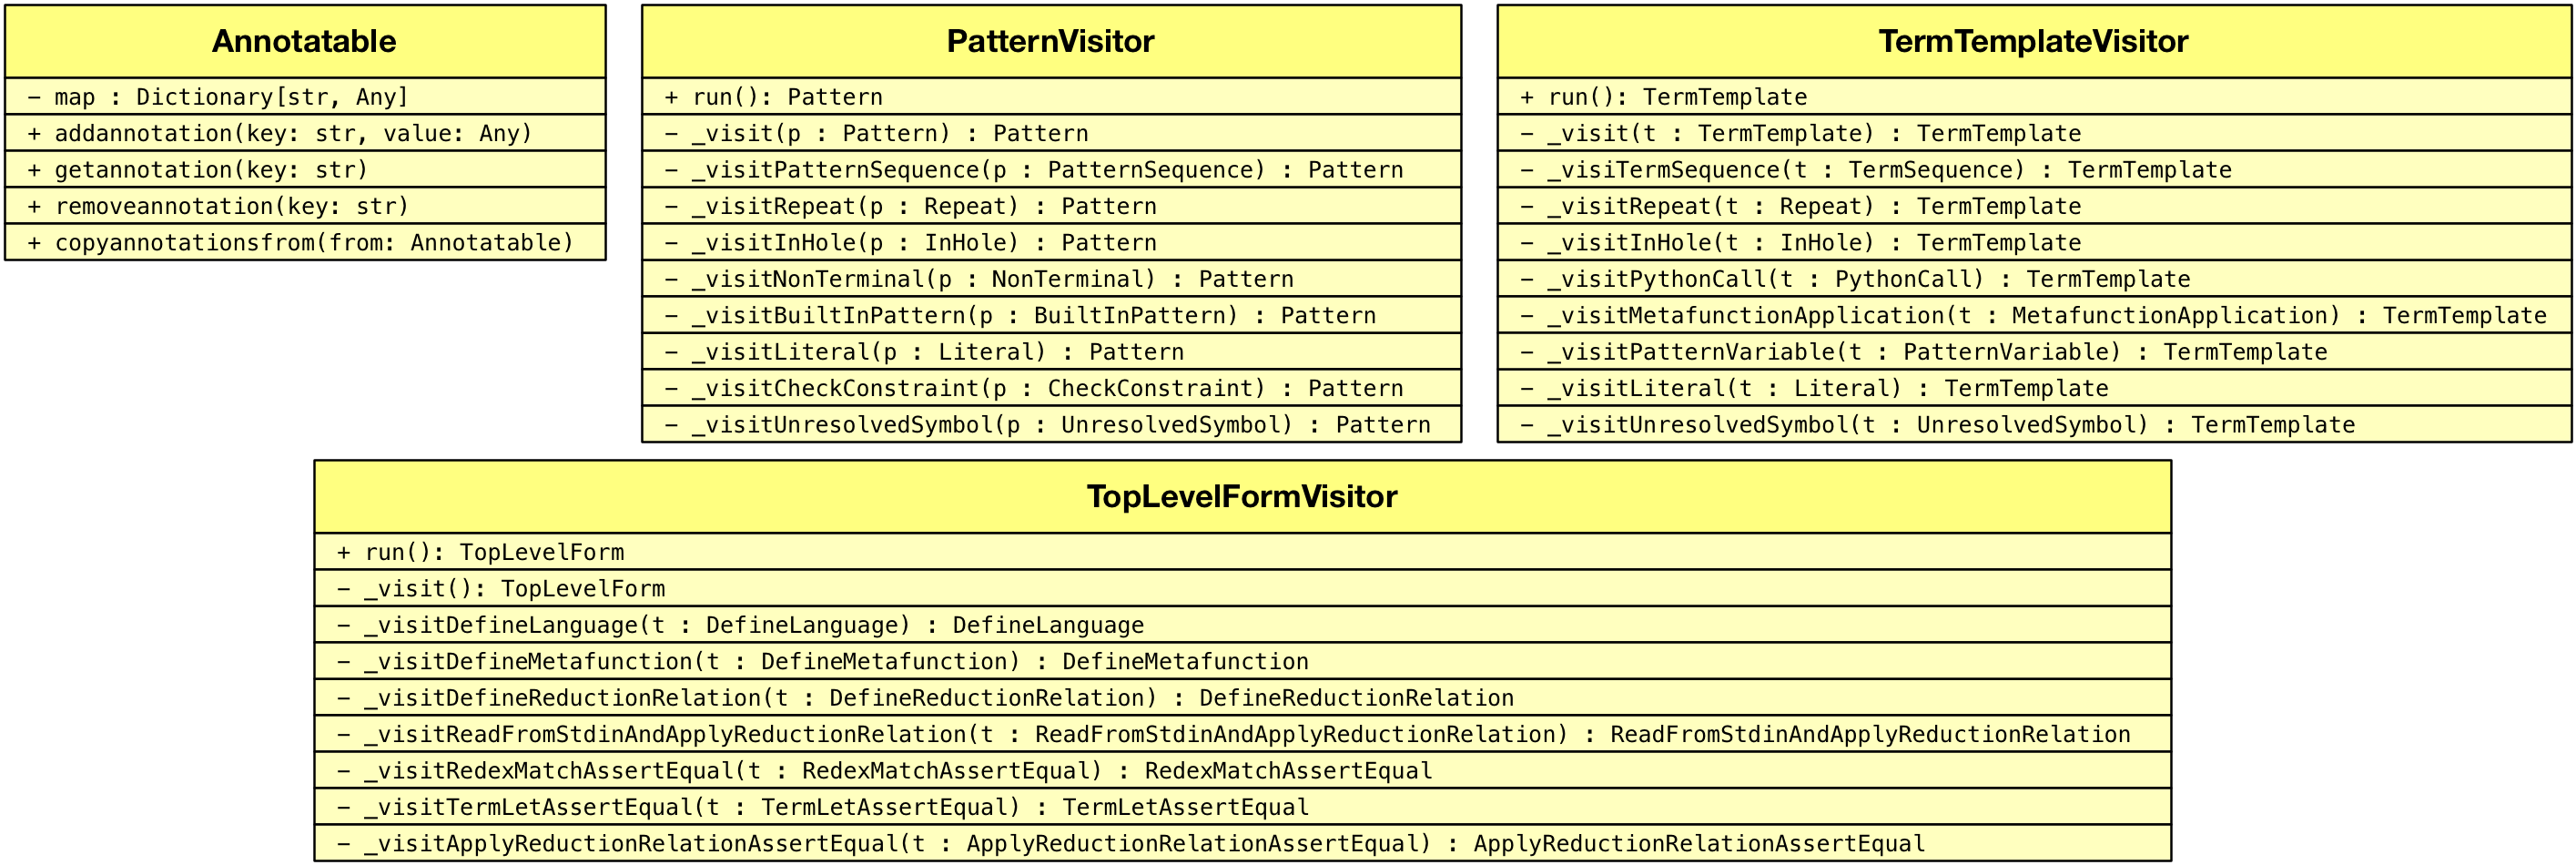
\includegraphics[scale=0.20]{class-diagram-visitors.png} }
	\caption{Representation of visitors and \texttt{Annotatable} class.}
\label{class-diagram-visitors}
\end{figure}

\FloatBarrier

